\documentclass[9pt,twocolumn,twoside]{../../styles/osajnl}
\usepackage{fancyvrb}
\journal{i524} 

\title{Automated Sharded MongoDB Deployment and Benchmarking for Big Data Analysis}

\author[1,*]{Mark McCombe}
\author[1,*]{Gregor von Laszewski}

\affil[1]{School of Informatics and Computing, Bloomington, IN 47408, U.S.A.}
\affil[*]{Corresponding author: mmccombe@iu.edu}

\dates{Project: S17-IO-3012, \today}

\ociscodes{MongoDB, Cloud Computing, Ansible, Python, Cloudmesh Client, OpenStack, I524}

% replace this with your url in github/gitlab
\doi{Report: \url{https://github.com/cloudmesh/sp17-i524/tree/master/project/S17-IO-3012/report/report.pdf}\\
Code: \url{https://github.com/cloudmesh/sp17-i524/tree/master/project/S17-IO-3012/code}}


\begin{abstract}

Using Python, Ansible, Bash Shell, and Cloudmesh Client a fully
automated process is created for deploying a configurable MongoDB
sharded cluster on Chameleon, FutureSystems, and Jetstream cloud
computing environments. A user runs a single Python program which
configures and deploys the environment based on parameters specified
for numbers of Config Server Replicas, Mongos Instances, Shards, and
Shard Replication. The process installs either MongoDB version 3.4 or
3.2 as requested by the user. Additionally, functionality exists to
run benchmarking tests for each deployment, capturing statistics in a
file as input for python visualization programs, the results of which
are displayed in this report. These reports depict the impact of
MongoDB version and degrees of sharding and replication on
performance. Key performance findings regarding version, sharding, and
replication are abstracted from this analysis. As background,
technologies and concepts key to the deployment and benchmarking, such
as MongoDB, Python, Ansible, Cloudmesh Client, and OpenStack are
examined.

\end{abstract}

\setboolean{displaycopyright}{true}

\begin{document}

\maketitle

\section{Introduction}

As the final project for I524, Big Data Software and Projects, Spring
2017, a Python program invoking Bash shell scripts, Ansible playbooks,
and Cloudmesh Client commands has been created to fully automate a
configurable deployment of a MongoDB sharded cluster on various
clouds. Chameleon Cloud, FutureSystems, and Jetstream are the
currently supported cloud environments. The scripts have been
developed and tested on an Ubuntu 16.04 LTS (Xenial Xerus) Virtual
Machine running in Virtual Box. Using the Python cmd command line
interface, the program project.py accepts parameters for deployment
cloud, MongoDB version, Config Server replication, number of Mongos
instances, number of Data Shards, and Shard replication.

Also via project.py, automated benchmarking tests can be run. Tests
were performed with various sharding and replication configurations to
assess their impact on performance. Additionally, tests were run
against MongoDB versions 3.4 and 3.2 to uncover any performance
differences between these version. Performance results are captured
and graphed using Python's matplotlib, the results of which are
displayed and analyzed in this report.

\section{Infrastructure}

Three clouds were selected for deployment: Chameleon Cloud,
FutureSystems (also referred to as Kilo in some sections of this
document), and Jetstream. In our automated deployment and benchmarking
process, the cloud name is passed as a parameter to the deploy
function of the main project.py script and a customized version of
MongoDB is deployed to the selected cloud.

\subsection{OpenStack}

Chameleon Cloud, FutureSystems and Jetstream all utilize OpenStack.
OpenStack is a free, open source cloud computing platform, primarily
deployed as IaaS \cite{www-wikiOpenStack}. OpenStack was created in
2010 as joint project between NASA and Rackspace that is currently
managed by the OpenStack Foundation \cite{www-wikiOpenStack}. Open
Stack is open source software released under the Apache 2.0 license
\cite{www-openStackFAQ}.

Open Stack has various components, also known by code names
\cite{www-wikiOpenStack}. Examples of OpenStack components (and code
names) are Compute (Nova), Networking (Neutron), Block Storage
(Cinder), Identity (Keystone), Image (Glance), Object Storage (Swift),
Dashboard (Horizon), Orchestration (Heat), Workflow (Mistral),
Telemetry (Ceilometer), OpenStack Telemetry (Ceilometer), Database
(Trove), Elastic Map Reduce (Sahara), Bare Metal (Ironic), Messaging
(Zaqar), Shared File System (Manila), DNS (Designate), Search
(Searchlight), and Key Manager (Barbican) \cite{www-wikiOpenStack}.

\subsection{Chameleon Cloud}

Chameleon is funded by the National Science Foundation and provides
computing resources to the open research community. The Chameleon
testbed is hosted at the Texas Advanced Computing Center and the
University of Chicago. Chameleon provides resources to facilitate
research and development in areas such as Infrastructure as a Service,
Platform as a Service, and Software as a Service. Chameleon provides
both an OpenStack Cloud and Bare Metal High Performance Computing
Resources \cite{www-chamAbout}.


\subsection{FutureSystems}

FutureSystems is a computing environment run by Indiana University
that supports educational and research activities
\cite{www-futureSystems}. FutureSystems is directed by Geoffrey C. Fox
and Gregor von Laszewski, both of Indiana University
\cite{www-futureSystems}. For our deployment, we utilize the OpenStack
Kilo Cloud, running on the India machine. Because the environment is
by default referred to as Kilo in the Cloudmesh documentation and
setup file, it is referred to as both FutureSystems and Kilo in
subsequent sections of this document and the accompanying diagrams.


\subsection{Jetstream}

Jetstream is a cloud computing environment implemented by many
academic and industry partners including the University of Texas at
Austin's Texas Advanced Computing Center (TACC), the Computation
Institute at the University of Chicago, the University of Arizona, the
University of Texas San Antonio, Johns Hopkins University, Penn State
University, Cornell University, the University of Arkansas at Pine
Bluff, the National Snow and Ice Data Center (NSIDC), the Odum
Institute at the University of North Carolina, the University of
Hawaii, and Dell \cite{www-jetstream1}. At Indiana University,
leadership is provided by the Pervasive Technology Institute with
involvement from several members of the School of Informatics and
Computing including Beth Plale, Katy Borner, and Volker Brendel
\cite{www-jetstream2}.


\subsection{Cloud Hardware Comparison}


Table \ref{tab:cloud-comparison} shows a comparison of key computing
resources on Chameleon, FutureSystems, and Jetstream cloud
environments.

\begin{table}[htbp]
\centering
\caption{\bf Cloud Hardware Specification Comparison \cite{www-chamHardware} \cite{www-kiloHardware} \cite{www-jetHardware}}

 \begin{tabular} {| c | c | c | c |}
\hline
  & FutureSystems &  Chameleon  & Jetstream \\ [0.5ex] 
 \hline

    
CPU     &  Xeon E5-2670 & Xeon X5550 & Haswell E-2680  \\
 \hline
cores   & 1024          &       1008 &  7680 \\
 \hline
speed   & 2.66GHz       &     2.3GHz & 2.5GHz\\
 \hline
RAM     & 3072GB        &    5376GB  &  40TBr\\
 \hline
storage & 335TB         &     1.5PB  & 2 TB\\ [1ex] 
 \hline

\end{tabular}
  \label{tab:cloud-comparison}
\end{table}

\section{Python/cmd}

Python is utilized in two portions of the automated process. First,
the main script, project.py, is a Python program that utilizes the cmd
module to provide a simple command line interface \cite{www-cmd}
accepting parameters for deployment configuration. project.py also
provides other functionality such as cluster deletion, benchmarking,
benchmarking summarization and reporting, and data distribution
reporting. Second, several visualization programs for benchmarking
analysis are written in Python, utilizing the matplotlib and pandas
modules.

\section{Ansible}

Ansible is open source software typically use to automate software
provisioning and configuration management. Ansible uses Playbooks
specified in YAML file format to accomplish this goal. Ansible runs on
Linux/Unix and requires Python \cite{www-wikiAnsible}.

In our deployment, virtual machines are created using Cloudmesh Client
cluster commands. Once they are created, all direct cloud interaction
for the MongoDB software installation and environment customization
and setup is performance via Ansible playbooks.



\section{Cloudmesh Client}

The Cloudmesh Client toolkit is an open source client interface that
standardizes access to various clouds, clusters, and workstations
\cite{www-cloudmesh}. Cloudmesh Client is a python based application
developed by Gregor von Laszewski and others collaborators primarily
at Indiana University.

In the deployment, Cloudmesh Client is used to handle most interaction
with the Virtual Machines in the clouds. Cloudmesh Client provides
functionality in three main areas: Key Management, OpenStack Security,
and virtual machine management. For key management, Cloudmesh's key
add and upload commands simplify secure interaction with the cloud
environments. For OpenStack security, Cloudmesh's secgroup commands
allow new security rules to be added and uploaded to the cloud.
Virtual machine management is performed with Cloudmesh's cluster
functionality, which allows easy creation and deletion of virtual
machines and communication between them.

Cloudmesh Client simplifies and standardized interaction with the
cloud for these tasks. This allows us to more easily port the
deployment to additional clouds that are supported by Cloudmesh.
Furthermore, by encapsulating the logic necessary to perform these
tasks we are shielded from changes in interfaces made by individual
clouds.

\section{MongoDB}

MongoDB is a popular open source, document oriented noSQL database. It
stores documents in JSON-like schema-less formats called collections
\cite{www-MonWiki}. DBEngines ranks MongoDB as the most popular noSQL
store and as the fifth most popular Database Management System overall
\cite{www-dbEngines}.

\subsection{Architecture}

A sharded cluster in MongoDB has three main components, all of which
will be implemented in our deployment:

\begin{itemize}
\item Config Servers - hold configurations setting and metadata
\item Mongos - a query routing interface between applications and the cluster
\item Shards - subsets of data
\end{itemize}

\begin{figure}[htbp]
\centering
\fbox{\includegraphics[width=\linewidth]{images/sharded-cluster-production-architecture.png}}
\caption{Sharded MongoDB Architecture \cite{www-mongoComponents}}
\label{fig:mongodb-arch}
\end{figure}


Figure \ref{fig:mongodb-arch} depicts a sharded MongoDB environment
with two Mongos instances and two data Shards. The replica sets shown
for both Config Servers and Shards may have any number of replicas
within the set.

\subsection{Config Servers}

Config Servers stored metadata for sharded MongoDB clusters. This
metadata includes information about the state and structure of the
data and components of the sharded cluster \cite{www-mongoConfig}.

Config Servers also contain authentication information. For example,
information about the key files used for internal authentication
between the nodes is stored in the Config Servers
\cite{www-mongoConfig}.

In production deployments, it is recommended for Config Servers to be
deployed in 3 member replica sets \cite{www-mongoComponents}. The
rationale behind a 3 member set is discussed in more detail in the
Replication subsection that follows.

In our deployment and benchmarking automation, the degree of
replication in the Config Server Replica Set is by the third parameter
to the main project.py script. For example, specifying 1 will create a
Replica Set with one Config Servers (not replication), specifying 3
will create a Replica Set with three Config Server, and so on.

\subsection{Mongos Routers}

Mongos is a query routing service used in sharded MongoDB
configurations. Queries from applications go through Mongos, which
locates the data in the sharded cluster. The Mongos instances
accomplish this by reading and caching data from the Config Servers
\cite{www-mongoMongos}.

For applications with high performance or availability requirements
multiple Mongos instances may be ideal. In a high volume application,
spreading the routing load over multiple Mongos instances can benefit
performance. Additionally, multiple Mongos instances may increase
availability in the case where a Mongos instance fails
\cite{www-mongoConfig}.

In our deployment and benchmarking automation, the number of Mongos
instances is controlled by the fourth parameter to the main project.py
script. For example, specifying 1 will create one Mongos instance,
specifying 3 will create three Mongos instances, and so on.


\subsection{Shards}

Sharding, or distributing data across machines, is used by MongoDB to
support large data sets and provide high throughput
\cite{www-sharding}. Our deployment and benchmarking will test the
performance of various numbers of shards, measuring the performance
improvements associated with sharding in MongoDB.

Documents are distributed among the shards using a shard key. A
sharded collection must have one, and only one, shard key which must
have a supporting index \cite{www-sharding}. Since the shard key is
critical to performance and efficiency, particular care must be given
to shard key selection \cite{www-shardkey}. In our performance testing
a key was chosen that would distribute data relatively evenly across
the shards, but was not used in retrieving the data as the more costly
retrieval of not using an index provided a better test case.


In our deployment and benchmarking automation, Sharding is controlled
by the fifth parameter to the main project.py script. For example,
specifying 1 cause only 1 shard to be created, specifying 3 will cause
three shards to be created, and so on.

\subsection{Replication}

In databases, replication provides data redundancy leading to greater
availability and fault tolerance. Replication in MongoDB is achieved
via Replica Sets \cite{www-replication}. Replica Sets were implemented
in our deployment for both Config Servers and Shards.

Two key benefits provided by replication are redundancy and fault
tolerance. Each Replica in a Replica Set provides another copy of
data. Higher redundancy means more nodes can be lost without data
being lost. Higher numbers of Replicas in a set also increase fault
tolerance, which leads to increased availability. As a general rule, a
set will be able to tolerate faults while the majority of its nodes
are still available


\begin{table}[htbp]
\centering
\caption{\bf Fault Tolerance by Replica Set Size \cite{www-mongoRepDep}}

 \begin{tabular}{|c | c | c|} 
 \hline
Replica Members &  Majority Needed & Fault Tolerance \\ [0.5ex] 
 \hline\hline
    
2 &	1 &	0 \\
 \hline
3 &	2 &	1 \\ 
 \hline
4 &	3 &	1 \\ 
 \hline
5 &	3 &	2 \\ 
 \hline
6 &	4 &	2\\ 
 \hline
7 &	4 &	3\\ 
 \hline
8 &	5 &	3\\ [1ex] 
 \hline

\end{tabular}
  \label{tab:fault-tolerance}
\end{table}


As shown in Table \ref{tab:fault-tolerance}, odd numbers of members in
a replica set are a better choice for fault tolerance. For example,
both a 3 and 4 replace set can only tolerate one member failing while
maintaining availability. This is because a majority of the members
must be available to maintain availability. In a 3 replica set the
majority is 2, so it can tolerate 1 member failing. In a 4 replica
set, the majority is 3, so it can still only tolerate 1 member
failing. Increases in fault tolerance only occur when the next odd
numbered member of a replica set is added \cite{www-mongoRepDep}.

For production systems, a standard deployment is a 3 Replica Set
\cite{www-mongoRepDep}. A 3 replica set provides 3 copies of the data
for redundancy and fault tolerance if 1 member of the set were to
fail. In a situation where availability was of higher concern, a 5
replica set would provide 4 copies of the data for redundancy and
fault tolerance if 2 members of the set were to fail.

In our automated deployment and benchmarking process, the degree of
replication for Shards is controlled by the sixth parameter to the
main project.py script. For example, specifying 1 for will create a
replica set per shard with only one copy of data (essentially no
replication, although technically we create a one member replica set),
specifying 3 will cause a replica set of with three copies to be
created, and so on.

\subsection{MongoDB Versions}

The most current version of MongoDB is version 3.4, which was released
on November 29, 2016. Based on an input parameter, our deployment will
install either version 3.4 or version 3.2, the prior version of
MongoDB. Many enhancements were made for version 3.4 impacting Sharded
Clusters, Replica Sets, Aggregation, Indexes, Views, Security, Tools,
and Platform Support. The complete list of 3.4 features and
enhancements can be found in the Release Notes
\cite{www-mongoRelease}.

In our automated deployment and benchmarking process, the version of
MongoDB installed is controlled by the second parameter to the main
project.py script. Specifying 34 will install version 3.4. Specifying
32 will install 3.2. These versions were selected as they are the two
most recent major versions of MongoDB and because they are the only
two compatible with Ubuntu 16.04 LTS (Xenial Xerus).

\subsection{Security}

There are two levels of security to consider in a sharded MongoDB
deployment: internal and external authentication.

In our deployment the various MongoDB components (config servers,
mongos instances, shards, and replicas) all reside on separate Virtual
Machines. These machines must be able to communicate with each other.
Two steps were necessary to enable this internal authentication.
First, the ports (27017, 27018, 27019, 28017) used by MongoDB needed
to be opened for communication. This was accomplished by adding
appropriate security group rules to the clouds through Cloudmesh
client. Second, MongoDB requires the internal authentication to be
done by either key files or x.509 certificates \cite{www-mongoAuth}.
In our deployment, authentication is done by key files. A new key file
is automatically created for each deployment and distributed to all of
the virtual machines on the selected cloud.

For external authentication, the three users are created. The user
\emph{admin} is created with the role of \emph{userAdminAnyDatabase}.
\emph{admin} performs administrative functions such as creating the
other users. The user \emph{cluster\_admin\_user} is created with the
role \emph{clusterAdmin}. \emph{cluster\_admin\_user} user performs
sharding functions such as sharding the collection and checking its
data distribution. \emph{user1} is a standard user with readWrite
permissions. \emph{user1} performs the benchmarking tests and other
functions not requiring administrative privileges.



\section{Deployment}


The automated process fully deploys a sharded MongoDB environment with
the Cloud, MongoDB version, number of Config Servers, Mongos
Instances, Shards, and degree of Replication specified as input
parameters.

\subsection{Computing Resources}

In all cases, virtual machines are deployed with the Ubuntu 16.04 LTS
(Xenial Xerus) operating system. On OpenStack the flavor or the
machine determines the amount of computing resources (CPU, memory,
storage) allocated to it. In our testing, m1.medium was used as the
flavor for Chameleon Cloud and FutureSystems, while m1.small was used
on Jetstream. Jetstream has more resources allocated to each flavor
than Chameleon and FutureSystems, which are similar. In order to
perform similar tests on each cloud, flavors with identical CPU and
memory were selected. Table \ref{tab:computing-resources} shows the
comparative resources of the flavors used in our testing. While
storage is lower on Jetstream, it is sufficient for out tests and
should not significantly impact performance.

\begin{table}[htbp]
\centering
\caption{\bf Computing Resources}

 \begin{tabular}{|c | c | c | c| c|} 
 \hline
 
Cloud &  Flavor & VCPU & RAM & Size \\ [0.5ex] 
 \hline
    
Chameleon &  m1.medium & 2 & 4 &	40 \\
 \hline
FutureSystems &  m1.medium &  2 &	4 &	40 \\ 
 \hline
Jetstream &  m1.small &  2 &	4 &	20 \\ 
\hline
\end{tabular}
  \label{tab:computing-resources}
\end{table}

\subsection{Deployment Process}

Several programs are involved in the deployment.  A high level overview of each is provided.

\subsubsection{project.py}

The deployment process is invoked by running the deploy function of
project.py, passing six required parameters: cloud (chameleon,
jetstream, or kilo), version (32 or 34 for version 3.2 or 3.4), size
of the config server replica set (a number, 1 or greater), number of
mongos routers (a number, 1 or greater), number of data shards (a
number, 1 or greater), and size of data shard replica sets.

Project.py calls a bash script, deploy.sh, which runs two bash shell
scripts to accomplish the deployment: cluster.sh and ansible.sh.

\subsubsection{cluster.sh}

Cluster.sh does the work of creating the cluster in the specified
cloud environment. First, it creates a key file needed for secure
access between the nodes, and uses Cloudmesh secgroup commands to
builds and uploads a new security group with the ports necessary for
MongoDB (27017, 27018, 27019, and 28017) accessible. Next, it uses
Cloudmesh client cluster commands to launch the appropriate number of
virtual machines in the desired cloud. Then, it builds a file,
inventory.txt, with sections for each MongoDB component (Config
Servers, Mongos Instances, and Shard Replica Sets), allocating the
correct number of IP addresses to each. Finally, cluster.sh builds a
few complex commands that will need to be run later in the process by
ansible.

\subsubsection{ansible.sh}

After the virtual machines have been created by cluster.sh, ansible.sh
used the inventory.txt file to execute Ansible playbooks on the
appropriate virtual machines.

\begin{enumerate}


\item install-python.yaml - Installs Python, if not installed.  This
script was necessary because the Ubuntu Zenial image on FutureSystems
does not have Python installed.  Python is required for Ansible.  

\item mongo-install32.yaml - Using apt\_key and apt\_repository,
installs the packages for version 3.2 of MongoDB on all virtual
machines.

\item mongo-install34.yaml - Using apt\_key and apt\_repository,
installs the packages for version 3.4 of MongoDB on all virtual
machines.

\item add-mongo-key.yaml - Uploads the key file created in cluster.sh
to all virtual machines.

\item mongo-config.yaml - On Config Servers only, stops the mongod
service and uses a template file to start the mongod process for a
Config Server.

\item mongo-config2.yaml - On only one Config Server, uses a template
file to initiate the primary Config Server.

\item mongo-mongos.yaml - On Mongos Instances only, stops the mongod
service and uses a template file to start the mongos process for a
Mongos instance.

\item mongo-users.yaml - On only one Mongos Instance, create several
users needed in later steps.

\item mongo-shard.yaml - On Shards only, stops the mongod service and
uses a template file to start the mongod process for a Shard.

\item mongo-shard2.yaml - On the primary Shard in each Replica Set,
uses a file built in cluster.sh to initiate the Shards.

\item add-shards.yaml - On one Mongos instance, uses a file built in
cluster.sh to add all of the Shards.

\item create-sharded-collection.yaml - Uploads several files to one
Mongos instance that will be need for benchmarking and shard the
collection (benchmarking setup, not included in deployment times).

\item getdata.yaml - Downloads and unarchive the pitches data from an
AWS S3 directory.  Also, create a smaller version for testing
(benchmarking setup, not included in deployment times). 

\end{enumerate}

The kill function in project.py will delete and deallocate the last
existing cluster on the cloud to clean up after the test is complete.


\subsection{Deployment Timing}

The configuration parameters and cluster and Ansible deployment times
are captured in a file for each deployment (benchmarking timings are
later captured as well). Total run time for a few interesting
configurations are shown in Table \ref{tab:deploy-times}.

Deployment A shows a simple deployment with only one of each component
being created. This deployment may only be suitable for a development
or test environment. Deployment A completed in 330 seconds.

Deployment B shows a more complex deployment with production like
replication factors for Config Servers and Shards and an additional
Mongos instance. This deployment may be suitable for a production
environment as it has greater fault tolerance and redundancy.
Deployment B took 1059 seconds to deploy.

Deployment C shows a deployment focused on high performance. It has a
high number of shards, nine, but no fault tolerance or redundancy. The
deployment may be suitable where performance needs are high and
availability is less critical. Deployment C finished in 719 seconds.


\begin{table}[htbp]
\centering
\caption{\bf Deployment Times on Chameleon Cloud in Seconds}

  \begin{tabular}{| c | c | c | c | c | c | c |} 
 \hline
 & Config &  Mongos & Shards & Replicas & Seconds \\

 
 \hline
 A & 1 & 1 & 1 & 1 & \emph{330} \\
 \hline
 B & 3 & 2 & 3 & 3 & \emph{1059} \\
 \hline
 C & 1 & 1 & 9 & 1 & \emph{719} \\ [1ex] 
 \hline


\end{tabular}
  \label{tab:deploy-times}
\end{table}

The total number of virtual machines is highly correlated with
deployment time as booting the machines and installing the software,
tasks that occur for all nodes, take the most time. The additional
steps to configure Config Servers, Mongos Instances, Replicas, and
Shards run in relatively similar times, so the specific type of
component created has little impact on the deployment time. For
example, holding all other deployment variables at 1, a deployment
with five Config Servers took 534 seconds, one with five Mongos
Instances took 556 seconds, one with five Shards took 607 seconds, and
one with a five Shard Replica set took 524 seconds. There is small
extra overhead to starting additional data shards, but a strong
correlation exists for total nodes to runtime for all configurations.
Deployment times for version 3.4 were very similar to version 3.2.

Table \ref{tab:deploy-times2} shows this empirically, as it takes a
very similar time to launch configurations with the same total number
of nodes, but extremely different mixed of Config Servers, Mongos
Instances, Replicas, and Shards.

The total number of nodes in a deployment can be calculated by the
following equation involving the parameters to the deployment script.

c + m + ( s * r ) = total nodes

\begin{table}[htbp]
\centering
\caption{\bf Deployment Times on Chameleon Cloud in Seconds}

 \begin{tabular}{| c | c | c | c | c | c |} 
 \hline
Config Servers &  Mongos & Shards & Replicas & Time in \\
-c &  -m & -s & -r & Seconds
\\ [0.5ex] 
 \hline
 \hline
\emph{5} & 1 & 1 & 1 & \emph{534} \\
 \hline
 1 & \emph{5}  & 1 & 1 & \emph{556} \\
 \hline
 1 & 1 & \emph{5} & 1 & \emph{607} \\
 \hline
 1 & 1 & 1 & \emph{5}  & \emph{524}  \\ [1ex] 
 \hline
\end{tabular}
  \label{tab:deploy-times2}
\end{table}

Due to Chameleon Cloud having the most reliable and consistent
performance of the three clouds, performance numbers are presented
only for selected runs on Chameleon. These numbers are proportionately
representative of deployment timings on Jetstream and FutureSystems.


\section{Benchmarking}

After the sharded MongoDB instance has been fully deployed, a
benchmarking process is run to assess performance of the
configuration. This process has also been fully automated. It is
invoked by running the benchmark function of project.py and passing
either the parameter large (for a full benchmark test) or small for a
small test.

\subsection{Data Set}

The data set used in the benchmarking testing and analysis was Major
League Baseball PITCHf/x data obtained by using the program Baseball
on a Stick (BBOS) \cite{www-bbos}. BBOS is a python program created by
\emph{willkoky} on github which extracts data from mlb.com and loads
it into a MySQL database. While it would be possible to convert this
program to populate the MongoDB database directly, collecting all of
the data is a time consuming process. Therefore, the data was captured
locally to the default MySQL database and then extracted to a CSV
file. This file contains 5,508,014 rows and 61 columns. It is
1,588,996,075 bytes in size uncompressed.


\subsection{Methodology}

There are several goals of the benchmarking process. The primary
benchmarking goal of the project is to assess the impact of sharding
on performance in MongoDB. Since replication was also built into the
deployment process, a secondary goal was to assess the impact of
replica sets on performance. A third goal is to assess performance of
MongoDB version 3.4 versus version 3.2, specifically for various shard
configuration. A final objective is to assess the relative performance
of the Chameleon, FutureSystems, and Jetstream cloud computing
environments.

The benchmarking tests are design to assess performance in three
situations: Reads, Writes, and MapReduce operations.



\subsubsection{Impact on Reads}

To access the impact of different configurations on writes, we use
MongoDB's mongoimport command. Mongoimport is a command line tool
capable of loading JSON, CSV, or TSV files \cite{www-mongoimport}. In
this case, we load a CSV file to the pitches collections in the mlb
database.

\subsubsection{Impact on Writes}

To assess the impact of different configurations on reads, we use
MongoDB's find command. We read the data previously loaded by the
mongoimport command to the pitches collection. The find command
retrieves documents that meet a specified criteria. In this case, we
search for pitches with a speed over 100 mph, a relatively rare event
in baseball. To limit the information sent back over the network, we
only return a count of these events. 3,632 is the count returned of
5,508,014 total documents. The column we search on does not have an
index, as the goal is to test the impact of sharding on a long running
query.

\subsubsection{Impact on MapReduce}

To assess the performance of MongoDB version, sharding, and
replication on reads, a simple MapReduce operation was written against
the pitches table to get the average speed of pitches that were stikes
versus those that were not strikes \cite{www-mapreduceEx}
\cite{www-mapreduce}.


\subsection{Benchmarking Process}

The benchmarking process is invoked by running the benchmark function
of the script project.py with the large parameter. Results for each
test are automatically captured in file benchmark\_datetime.csv. This
file included the configuration the test was run under (cloud, MongoDB
version, config server replication factor, mongos instances, number of
shards, and shard replication factor) along with the run times of the
find, mongoimport, and MapReduce commands. After all tests were run, a
shell script, combine\_benchdeploy.sh combines all files into one
file, benchmark\_combined.csv.

The graphical depictions of the test results shown in the next section
were created by running python programs to average the run times
across the shard, replication, and version configurations shown. For
consistency, config server replication and mongos instances were both
kept at one for all benchmarking tests. Additionally, replication was
kept at one for sharding and version tests and sharding at one for
replication tests. This methodologies allows us to isolate the
variable we are assessing. All sharding tests were run with one, two,
three, five, seven, and nine shards. All replication tests were run
with one, two, three, five, and seven replicas.


To setup for the test, a compressed version of file has been stored in
an Amazon Web Services S3 directory. This file is pre=staged on a
Mongos instance during the deployment (but excluded from the run time)
and is loaded it to a collection named \emph{pitches} in MongoDB using
mongoimport before running the find and MapReduce commands.


Before the benchmarking process can be run, a sharded collection must
be created and sharded. This was also done via Ansible during the
deployment in preparation for benchmarking. For reproducibility of
benchmarks, the benchmarking process also deletes any data from the
pitches collection that may have been loaded prior to running
mongoimport.


The shard key for the pitches table is set to pitchID. PitchID is a
unique key to each pitch document. Selecting pitchID as the shard key
should cause the data to be reasonably evenly distributed among the
shards. Data distribution will be analyzed in a subsequent section.




\subsection{Data Distribution}

To explore how data was allocated among the shards, a function called
distribution was built into project.py. This function runs the
getShardDistribution() command, which reports on how data and
documents are distributed among shards \cite{www-shardDist}. Tables
\ref{tab:data-dist32} and \ref{tab:data-dist34} show the results of
tests with one, three, and five shards in version 3.2 and 3.4 of
MongoDB. The results clearly show the data is well distributed,
although interestingly, in all cases there is some minor skew toward
the first shard having the most data. These results clearly show that
data distribution is similar in both versions of MongoDB.


\begin{table}[htbp]
\centering
\caption{\bf Data Distribution among Shards - Version 3.2}

 \begin{tabular}{| c | c | c | c | c | c |} 
 \hline
  &  1    &  2    &  3    &   4   & 5 \\ [0.5ex]
\hline
  \hline
1 & 100   &       &       &       &   \\
\hline
3 & 35.84 & 32.18 & 31.96 &       &   \\
\hline
5 & 23.04 & 19.27 & 19.40 & 19.38 & 18.89   \\
\hline
\end{tabular}
  \label{tab:data-dist32}
\end{table}



\begin{table}[htbp]
\centering
\caption{\bf Data Distribution among Shards - Version 3.4}

 \begin{tabular}{| c | c | c | c | c | c |} 
 \hline
  &  1    &  2    &  3    &   4   & 5 \\ [0.5ex]
\hline
  \hline
1 & 100   &       &       &       &   \\
\hline
3 & 36.23 & 31.82 & 35.75 &       &   \\
\hline
5 & 22.26 & 19.67 & 19.42 & 19.37 & 19.26   \\
\hline
\end{tabular}
  \label{tab:data-dist34}
\end{table}






\subsection{Benchmarking Analysis}


\subsubsection{Cloud Analysis}

Chameleon Cloud was significantly more stable and reliable than
FutureSystems and Jetstream Clouds for our testing. Chameleon yields
the fastest and most consistent results with very few errors.
Jetstream initially had stability problems that were eventually
resolved by the Jetstream support team. Once these issues were
resolved, Jetstream performance and stability was very close to
Chameleon's. FutureSystem performance was the poorest with respect to
run time. Environmental errors were initially frequent, but after
allocating new floating IPs test would be completed successfully.
JetStream performance was good, but the environment was very unstable.
Due to its stability and performance, Chameleon was chosen as the
environment to test MongoDB version 3.4 versus 3.2, due to its
stability.

\subsubsection{Impact of Sharding on Reads}


gure \ref{fig:shard-find} depicts the impact on performance of various
numbers of shards on a find command in Chameleon, FutureSystems, and
Jetstream Clouds. All three clouds show a strong overall decline in
run time as the number of shards increases, which shows the positive
impact of sharding on performance. For all clouds, reads were over 35
seconds for one shard and less than 10 seconds for five shards. This
is a significant gain in performance.

\begin{figure}[htbp]
\centering
\fbox{\includegraphics[width=\linewidth]{images/shard_find.png}}
\caption{Find Command - Sharding Test}
\label{fig:shard-find}
\end{figure}


All three clouds show a particularly large gain in performance when in
increasing from one shard to two. Run time for two shards is less than
one third the run time of one shard. Increases in shards beyond two
show much smaller incremental gains.

Perfomance on Chameleon Cloud and Jetstream is very similar for the
find test. Kilo performance is worse, although proportionately better
than on the mongoimport test. This is an interesting observation as
for both deployment and mongoimport, performance was much better on
Chameleon and FutureSystems than Kilo. One difference from the
mongoimport test is that much less data is being sent over the
network. Network speeds could be a factor in this discrepancy.

Figure \ref{fig:shard-find} can be recreated by running the program
benchmark\_shards\_find.py passing the file benchmark\_combined.csv as
a parameter. It plots the average run time for each configuration as
shown using matplotlib. This report is run automatically by the report
function of project.py.




\subsubsection{Impact of Sharding on Writes}




Figure \ref{fig:shard-import} depicts the impact on performance of
various numbers of shards on a mongoimport command in the three
clouds. For all clouds, run time of the mongoimport command in our
tests does not appear to be impacted by the number of shards. Since
the same amount of data is written with more computing resources
available when there are more shards, we might expect to see a
performance gain. However, there are possible explanations for
performance not improving. First, the mongoimport command may not
write data in parallel. This is not indicated in the documentation,
but it seems likely that it reads the file serially. Second, resources
on the server the data is written to may not be the bottleneck in the
write process. Other resources like the network time seem more likely
to be the bottleneck. Since we are always going over the network from
the mongos instance to a data shard, regardless of the number of
shards, a bottleneck in the network would impact all shard
configurations equally.

\begin{figure}[htbp]
\centering
\fbox{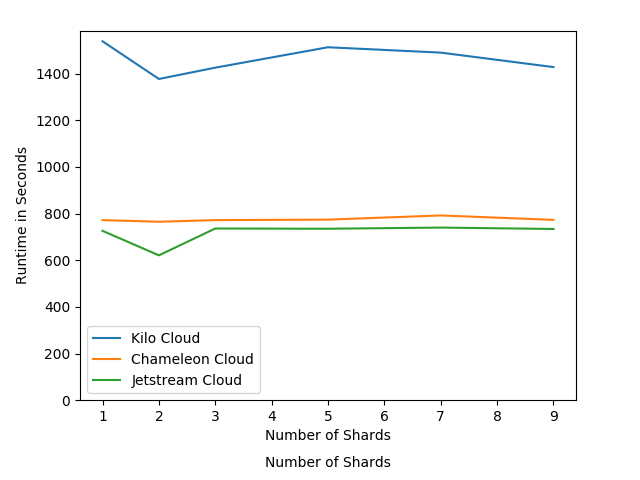
\includegraphics[width=\linewidth]{images/shard_import.png}}
\caption{Mongoimport Command - Sharding Test}
\label{fig:shard-import}
\end{figure}

While sharding did not benefit a single threaded mongoimport command,
it is likely it would benefit other heavy write operations,
particularly coming through multiple mongos instances. In a
non-sharded environment, this would lead to a heavy load on the single
data shard. In a sharded environment, the load on each shard would
drop as the number of shards increased.

While performance on Chameleon and FutureSystems was very similar for
the find command, performance of the mongoimport command was
significantly better on Chameleon than on Kilo. We see approximately
50\% better performance on both Chameleon and Jetstream Clouds
compared to FutureSystems. Jetstream performance is slightly better
than Chameleon for the import test.

Figure \ref{fig:shard-import} can be recreated by running the program
benchmark\_shards\_import.py passing the file benchmark\_combined.csv
as a parameter. It plots the average run time for each configuration
as shown using matplotlib. This report is run automatically by the
report function of project.py.

\subsubsection{Impact of Sharding on MapReduce}



Figure \ref{fig:shard-mapreduce} shows the performance of MapReduce
across various sharding configurations on our three clouds. These
results are relatively similar to the find results. While results are
inconsistent, particularly on FutureSystems, likely due to
environmental issues, all clouds show an overall decrease in
processing time with addition of shards. Relative to mongoimport
performance, performance is more similar across the three clouds for
MapReduce.

\begin{figure}[htbp]
\centering
\fbox{\includegraphics[width=\linewidth]{images/shard_mapreduce.png}}
\caption{MapReduce - Sharding Test}
\label{fig:shard-mapreduce}
\end{figure}


Figure \ref{fig:shard-mapreduce} can be recreated by running the
program benchmark\_shards\_mapreduce.py passing the file
benchmark\_combined.csv as a parameter. It plots the average run time
for each configuration as shown using matplotlib. This report is run
automatically by the report function of project.py.

\subsubsection{Impact of Replication on Reads}



Figure \ref{fig:replica-find} depicts the impact on performance of
various numbers of replicas on a find command in Chameleon,
FutureSystems, and Jetstream Clouds. These results show no correlation
between the number of replicas and find performance.

\begin{figure}[htbp]
\centering
\fbox{\includegraphics[width=\linewidth]{images/replica_find.png}}
\caption{Find Command - Replication Test}
\label{fig:replica-find}
\end{figure}

Similarly to other tests, performance on Chameleon was best for the
majority of the test runs in the find replication test, followed by
Jetstream, with FutureSystems performing the worst.

Figure \ref{fig:replica-find} can be recreated by running the program
benchmark\_replicas\_find.py passing the file benchmark\_combined.csv
as a parameter. It plots the average run time for each configuration
as shown using matplotlib. This report is run automatically by the
report function of project.py.



\subsubsection{Impact of Replication on Writes}


\begin{figure}[htbp]
\centering
\fbox{\includegraphics[width=\linewidth]{images/replica_import.png}}
\caption{Mongoimport Command - Replication Test}
\label{fig:replica-import}
\end{figure}


Figure \ref{fig:replica-import} depicts the impact on performance of
various numbers of replicas on a mongoimport command on our three
Clouds. The results show poorer write performance as the number of
replicas increase. Given that an extra copy of data is written with
each increase in the replication factor, this performance hit is
expected.




Performance on Jetstream and Chameleon were very close on this test
with Chameleon only performing significantly better with four or more
replicas. FutureSystems import performance was by far the worst of the
three clouds.

Figure \ref{fig:replica-import} can be recreated by running the
program benchmark\_shards\_import.py passing the file
benchmark\_combined.csv as a parameter. It plots the average run time
for each configuration as shown using matplotlib. This report is run
automatically by the report function of project.py.


\subsubsection{Impact of Replication on MapReduce}

\begin{figure}[htbp]
\centering
\fbox{\includegraphics[width=\linewidth]{images/replica_mapreduce.png}}
\caption{MapReduce - Replication Test}
\label{fig:replica-mapreduce}
\end{figure}

As shown in Figure \ref{fig:replica-mapreduce}, replication appears to
have no impact on MapReduce operations. While there are variations in
FutureSystems and Jetstream performance for different numbers of
replicas, they do not follow a consistent pattern and appear to be
caused by environmental issues. This is an interesting result as
increased levels of replication came with a performance penalty for
the find commmand, which also reads data.

As with several other tests, Chameleon MapReduce performance was the
best, followed by Jetstream, with FutureSystems again being the worst.

Figure \ref{fig:replica-mapreduce} can be recreated by running the
program benchmark\_shards\_import.py passing the file
benchmark\_combined.csv as a parameter. It plots the average run time
for each configuration as shown using matplotlib. This report is run
automatically by the report function of project.py.





\subsubsection{Impact of Version and Sharding on Reads}


\begin{figure}[htbp]
\centering
\fbox{\includegraphics[width=\linewidth]{images/version_find.png}}
\caption{Find Command - Version 3.2 vs 3.4}
\label{fig:version-find}
\end{figure}

Figure \ref{fig:version-find} shows the MongoDB version 3.4 and 3.2
find performance on Chameleon Cloud. Results are very close, with
version 3.2 having the best performance for one shard and performance
being similar for all other sharding levels.

Figure \ref{fig:version-find} can be recreated by running the program
benchmark\_version\_find.py passing the file benchmark\_combined.csv
as a parameter. It plots the average run time for each configuration
as shown using matplotlib. This report is run automatically by the
report function of project.py.

\subsubsection{Impact of Version and Sharding on Writes}

\begin{figure}[htbp]
\centering
\fbox{\includegraphics[width=\linewidth]{images/version_import.png}}
\caption{Mongoimport Command - Version 3.2 vs 3.4}
\label{fig:version-import}
\end{figure}


Figure \ref{fig:version-import} shows the MongoDB version 3.4 and 3.2
mongoimport performance on Chameleon Cloud. Runtimes are similar for
each version. Version 3.2 is slightly faster at the lowest sharding
levels and Version 3.4 is slightly faster at the highest sharding
level. Given the mixed results and close run times, neither version
shows a significant advantage for write operations.

Figure \ref{fig:version-import} can be recreated by running the
program benchmark\_version\_find.py passing the file
benchmark\_combined.csv as a parameter. It plots the average run time
for each configuration as shown using matplotlib. This report is run
automatically by the report function of project.py.



\subsubsection{Impact of Version and Sharding on MapReduce}

Figure \ref{fig:version-mapreduce} shows the MongoDB version 3.4 and
3.2 mongoimport performance on Chameleon Cloud. Runtimes are similar
for each version and with each version being faster at some shard
level, which appears to be random. Given the mixed results and close
run times, neither version shows a significant advantage for MapReduce
operations.

\begin{figure}[htbp]
\centering
\fbox{\includegraphics[width=\linewidth]{images/version_mapreduce.png}}
\caption{MapReduce - Version 3.2 vs 3.4}
\label{fig:version-mapreduce}
\end{figure}

Figure \ref{fig:version-mapreduce} can be recreated by running the
program benchmark\_version\_find.py passing the file
benchmark\_combined.csv as a parameter. It plots the average run time
for each configuration as shown using matplotlib. This report is run
automatically by the report function of project.py.



\section{Summary}

We have created, tested, and demonstrated a fully automated program to
configure and deploy a sharded MongoDB cluster to three cloud
environments: Chameleon, Jetstream, and FutureSystems. Using a
combination of Python, Bash, and Cloudmesh Client, the a cluster is
dynamically deployed with a selected number of Config Server Replicas,
Mongos Routers, Shards, and Shard Replicas and either MongoDB version
3.4 or 3.2. Functions also exist for terminating the environment,
reporting on data distribution, benchmarking, and reporting on
performance testing.

An automated benchmarking process to show the impact of well
distributed data across shards of a large data set has been run for
various configurations. The impact of MongoDB version 3.4 versus 3.2,
Sharding, and Replication on performance have been assessed. Testing
showed performance and stability on Chameleon Cloud to be the best of
our three cloud environments with Jetstream a close second after an
environmental issue was resolved by the support team. FutureSystems
performance consistently lagged behind the other two clouds. A key
finding is that read performance, typically a high priority for noSQL
data stores and Big Data operations, increases significantly as shards
are added. Testing also showed that a predictable performance penalty
is associated with replication. Our comparison of version 3.4 and 3.2
showed no significant differences between version 3.2 and 3.4
performance across various sharding levels.

\section*{Acknowledgements}

This work wos conducted with the help of resources provided by
FutureSystems and Chameleon Cloud.

% Bibliography

\bibliography{references}
 
\section*{Author Biographies}
\begingroup
\setlength\intextsep{0pt}
\begin{minipage}[t][3.2cm][t]{1.0\columnwidth} % Adjust height [3.2cm] as required for separation of bio photos.
  \noindent
{\bfseries Mark McCombe} received his B.S. (Business Administration/Finance) and M.S. (Computer Information Systems) from Boston University.  He is currently studying Data Science at Indiana University Bloomington.

\end{minipage}
\endgroup

\newpage

\appendix

\section{Code References}
References used in deployment, benchmarking, visualization programs are formally documented here as well as noted in a comment in the code \cite{www-bashNum} \cite{www-lastChar} \cite{www-configOpts} \cite{www-bashArgs} \cite{www-cmVms}  \cite{www-python1}  \cite{www-python2}  \cite{www-python3} \cite{www-ansibleDir} \cite{www-mongoAnsible} \cite{www-ansibleCopy} \cite{www-ansibleHost} \cite{www-installMongo} \cite{www-ansiblePython}.

\section{Execution Instructions}

The project should be run on an Ubuntu 16.04 LTS (Xenial Xerus)
machine. The required modules for the project can be installed in a
virtualenv virtual environment using the file
project/S17-IO-3012/code/requirements.txt.

The main script, project/S17-IO-3012/code/bin/project.py, can be run
to execute all functionality. Project.py functions (deploy, kill,
benchmark, report, distribution) are described in help, but sample
instructions are provided below for each function.

python project.py has four functions.

\subsection{deploy}

Runs a deployment.  Takes 6 parameters:


\begin{enumerate}

\item Cloud - chameleon, jetstream, or kilo (futuresystems)
\item MongoDB Version - 34 for version 3.4, 32 for version 3.2
\item Config Server Replication Size - a number
\item Mongos Router Instances - a number
\item Shard Count - a number
\item Shard Replication Size - a number


\end{enumerate}

Simple example:

deploy chameleon 34 1 1 1 1

More complex examples: 

deploy chameleon 32 3 2 3 3

deploy kilo 34 2 2 1 1


\subsection{kill} - Deletes and undefines the current cluster.  No parameters.

\subsection{benchmark}

Runs a benchmark mongoimport, find, and MapReduce and logs timings.
Takes one required parameter - \emph{large} or \emph{small} (for
testing purposes).

\subsection{report}

Regenerates PNG files in the code/report/directory based on current
benchmarks

\subsection{distribution}

Shows the data distribution of the current configuration. For
meaningful results, must be run after benchmark.

\section{Directory Structure}

The project/S17-IO-3012/code contains several directories.   

\subsection{benchmark/} Contains all benchmark timing logs  
\subsection{bin/} Contains all Bash and Python code
\subsection{configfiles/} Contains all configuration file templates
\subsection{deploy/} Contains all deployment timing logs
\subsection{json/} Contains all json documents
\subsection{playbooks/} Contains all Ansible YAML files 
\subsection{report/} Contains all reports in PNG format
\subsection{stdlist/} Contains all bash script output logs
\subsection{work/} Contains temporary work files

\end{document}
